\chapter{\label{ecm-rcm}The ECM and RCM Contention Managers}
\markright{Mohammed El-Shambakey \hfill Chapter~\ref{ecm-rcm}. ECM and RCM \hfill}
%
We consider software transactional memory (STM) for concurrency control in multicore embedded real-time software. We investigate real-time contention managers (CMs) for resolving transactional conflicts, including those based on dynamic and fixed priorities, and establish upper bounds on transactional retries and task response times. We identify the conditions under which STM (with the proposed CMs) is superior to lock-free synchronization~\cite{stmconcurrencycontrol:emsoft11} and real-time locking protocols (i.e., OMLP\cite{springerlink:10.1007/s10617-012-9090-1,key-3} and RNLP\cite{6257574}).

The rest of this Chapter is organized as follows, Section~\ref{sec:g-edf-edf-cm} investigates Earliest Deadline Contention Manager under G-EDF scheduling (ECM) and illustrates its behaviour. We provide computations of workload interference and retry cost analysis under ECM. Section~\ref{sec:g-rma-rma-cm} presents Rate Monotonic Contention Manager under G-RMA scheduling (RCM). It also includes retry cost and response time analysis under RCM. Schedulability of ECM and RCM is compared against schedulability of lock-free in Section~\ref{sec:comparison} and real-time locking protocols in Section~\ref{sec:stm_vs_locking}. We conclude the Chapter in Section~\ref{sec:ecm-rcm-conclusions}.
%
\section{ECM}
\label{sec:g-edf-edf-cm}
%
Since only one atomic section among many that share the same object can commit at any time under STM, those atomic sections execute in sequential order.  A task $\tau_{i}$'s atomic sections are interfered by other tasks that share the same objects with $\tau_{i}$. Hereafter, we will use \emph{ECM} to refer to a multicore system scheduled by G-EDF and resolves STM conflicts using the EDF CM. ECM was originally introduced in~\cite{6045438}. ECM will abort and retry an atomic section of $\tau_i^x$, $s_i^k$ due to a conflicting atomic section of $\tau_j^y$, $s_j^l$, if the absolute deadline of $\tau_j^y$ is less than or equal to the absolute deadline of $\tau_i^x$. ECM behaviour is shown in Algorithm~\ref{ecm_algorithm}. \cite{6045438} assumes the worst case scenario for transactional retry occurs when conflicting transactions are released simultaneously.~\cite{6045438} also assumes all transactions have the same length. Here, we extend the analysis in~\cite{6045438} to a more worse conflicting scenario and consider distinct-length transactions. We also consider lower number of conflicting instances of any job $\tau_j^y$ to another job $\tau_i^x$.
%
\begin{algorithm}
\footnotesize{
\LinesNumbered
\KwData{$s_i^k\rightarrow$ interfered atomic section. $s_j^l\rightarrow$ interfering atomic section}
\KwResult{which atomic section aborts}
\eIf{$d_i^k < d_j^l$}
	{$s_j^l$ aborts\label{ecm:step_sicommits}\;}
	{$s_i^k$ aborts\label{ecm:step_siaborts}\;}
	}
\caption{ECM}
\label{ecm_algorithm}
\end{algorithm}
%
\subsection{Illustrative Example}\label{ecm_illustrative_ex}
Behaviour of ECM can be illustrated by the following example:
\begin{itemize}
\item Transaction $s_{i}^{k}\in\tau_{i}^{x}$ begins execution.
Currently, $s_{i}^{k}$ does not conflict with any other transaction.
\item Transaction $s_{j}^{l}\in\tau_{j}^{y}$ is released while
$s_{i}^{k}$ is still running. $\Theta_i^k \cap \Theta_j^l \neq \emptyset$. $d_{j}^{y}<d_{i}^{x}$. So,
$p_{j}^{y}>p_{i}^{x}$. Hence, ECM will abort and restart $s_{i}^{k}$
in favour of $s_{j}^{l}$.
\item Transaction $s_{h}^{v}\in\tau_{h}^{u}$ is released while
$s_{j}^{l}$ is still running. $d_{h}^{u}<d_{j}^{y}<d_{i}^{x}$.
So, $p_{h}^{u}>p_{j}^{y}>p_{i}^{x}$. $s_{j}^{l}$ and $s_{i}^{k}$
will abort and retry until $s_{h}^{v}$ commits.
\item $s_{h}^{v}$ commits. $s_{j}^{l}$ executes while
$s_{i}^{k}$ aborts and retries.
\item $s_{j}^{l}$ commits. $s_{i}^{k}$ executes.
\end{itemize}
%
\subsection{Transitive Retry}\label{subsec:ecm_transitive_retry}
%
With multiple objects per transaction, ECM will face transitive retry, which we illustrate with an example.

\textbf{Example 1.} Consider three atomic sections $s_{1}^{x}$, $s_{2}^{y}$, 
and $s_{3}^{z}$ belonging to jobs $\tau_{1}^{x}$,$\tau_{2}^{y}$, 
and $\tau_{3}^{z}$, with priorities $p_{3}^{z}>p_{2}^{y}>p_{1}^{x}$, respectively. 
Assume that $s_{1}^{x}$ and $s_{2}^{y}$ share objects, $s_{2}^{y}$ and $s_{3}^{z}$
share objects. $s_{1}^{x}$ and $s_{3}^{z}$ do not share objects.
$s_{3}^{z}$ can cause $s_{2}^{y}$ to retry, which in turn will cause $s_{1}^{x}$ to retry. 
This means that $s_{1}^{x}$ may retry transitively
because of $s_{3}^{z}$, which will increase the retry cost of $s_{1}^{x}$.

Assume another atomic section $s_4^f$ is introduced. Priority of $s_4^f$ is higher than priority of $s_3^z$. $s_4^f$ shares objects only with $s_3^z$. Thus, $s_4^f$ can make $s_3^z$ to retry, which in turn will make $s_2^y$ to retry, and finally, $s_1^x$ to retry. Thus, transitive retry will move from $s_{4}^{f}$ to $s_{1}^{x}$, increasing the retry cost of $s_{1}^{x}$. 
The situation gets worse as more tasks of higher priorities are added, where each task
shares objects with its immediate lower priority task. $\tau_{3}^{z}$
may have atomic sections that share objects with $\tau_{1}^{x}$,
but this will not prevent the effect of transitive retry due to $s_{1}^{x}$.

\begin{mydef}
\textbf{Transitive(indirect) Retry:} A transaction $s_{i}^{k}$ suffers from
transitive retry when it conflicts with a higher priority transaction
$s_{j}^{l}$, which in turn conflicts with a higher priority transaction
$s_{z}^{h}$, but $s_{i}^{k}$ does not conflict with $s_{z}^{h}$.
Still, when $s_{j}^{l}$ retries due to $s_{z}^{h}$, $s_{i}^{k}$
also retries due to $s_{j}^{l}$. Thus, the effect of the higher priority
transaction $s_{z}^{h}$ is transitively moved to the lower priority
transaction $s_{i}^{k}$, even when they do not conflict on common objects.
\end{mydef}

\begin{clm}\label{ecm-rcm-transitive-retry}
ECM suffers from transitive retry for multi-object transactions.
\end{clm}
%
\begin{proof}\normalfont
%
ECM depends on priorities to resolve conflicts between transactions. Thus, lower priority transaction must always be aborted for a conflicting higher priority transaction. Claim follows.
%
\end{proof}
%
Because of transitive retry, $\Theta_i$ for any $\tau_i$ is extended to include any object $\theta \not \in \Theta_i$, but $\theta$ can make at least one transaction $s_i^k \in \tau_i$ retry transitively. The new set of objects that can cause direct or indirect retry of at least one transaction in $\tau_i$ is denoted as $\Theta_i^{ex}$. $\Theta_i^{ex}$ is obtained by being initialized to $\Theta_i$ (i.e., the set of objects that are already accessed by any transaction $s_i^k \in \tau_i$). We then cycle through all transactions belonging to all other higher priority tasks. Each transaction $s_j^l$ that accesses at least one of the objects in $\Theta_i^{ex}$ adds all other objects accessed by $s_j^l$ to $\Theta_i^{ex}$. The loop over all higher priority tasks is repeated, each time with the new $\Theta_i^{ex}$, until there are no more transactions accessing any object in $\Theta_i^{ex}$. However, this solution may over-extend the set of conflicting objects, and may even contain all objects accessed by all tasks. $\Theta_i^*$ represent the set of objects not accessed directly by any transaction in $\tau_i$, but any $\theta \in \Theta_i^*$ can make at least one transaction in $\tau_i$ retry transitively. Thus, $\Theta_i^{ex}=\Theta_i + \Theta_i^*$. Similarly, the distinct set of objects that can make $s_i^k$ retry directly or indirectly(transitively) is denoted as $\Theta_i^{k^{ex}}$. $\gamma_i$ is the extended to $\gamma_i^{ex}$. While $\gamma_i$ is the set of tasks- other than $\tau_i$- that access at least one object $\theta \in \Theta_i$, $\gamma_i^{ex}$ is the set of tasks- other than $\tau_i$- that access at least one object $\theta \in \Theta_i^{ex}$.
%
\subsection{\label{sec:g-edf interference and workload}G-EDF Interference}
%
\begin{clm}\label{clm:max_job_no_exist_j_interval_r}
%
Regardless of the used scheduler, maximum number of jobs of $\tau_{j}$
that can exist in time interval $L$ is upper bounded by 
\begin{equation}
\left\lceil\frac{L}{T_{j}}\right\rceil+1\label{eq:max_job_no_exist_j_interval_r}
\end{equation}
where at most two jobs $\tau_{j}$ can be partially included in $L$.
The remaining jobs of $\tau_{j}$ are totally included in $L$.
%
\end{clm}
%
\begin{proof}
%
Generally, $L=aT_{j}+b$, $0\le b<T_{j}$. $a$ is the maximum number
of jobs of $\tau_{j}$ that contribute by their minimum periods $T_{j}$
during $L$. If $b\ge T_{j}$, then there are more than $a$ jobs
of $\tau_{j}$ contributing by their minimum periods $T_{j}$ during
$L$, which contradicts definition of $a$. The remaining interval
$b(=L-aT_{j},\, b>0)$ can be divided between at most two jobs of
$\tau_{j}$. If $b$ can be divided between more than two jobs of
$\tau_{j}$, then there is more than $a$ jobs of $\tau_{j}$ that
contribute by their minimum periods $T_{j}$ during $L$. This contradicts
definition of $a$. So, if $b>0$, then maximum number of jobs of
$\tau_{j}$ that can exist during $L$ is $a+2=\left\lceil \frac{L}{T_{j}}\right\rceil +1$
.

If $b=0$, then jobs of $\tau_{j}$ can be shifted to the left or
the right during $L$. This results in $a+1$ jobs of $\tau_{j}$
during $L$. So, if $b=0$, then maximum number of jobs of $\tau_{j}$
that can exist during $L$ is $a+1=\left\lceil \frac{L}{T_{j}}\right\rceil +1$.
Claim follows. 
%
\end{proof}
%
\begin{clm}\label{clm:gedf_max_job_no_interfer_j_i}
%
Let $T_{i}=aT_{j}+b$, where $a=\left\lfloor\frac{T_i}{T_j}\right\rfloor$ and $0\le b<T_{j}$. Under G-EDF scheduler, maximum
number of jobs of $\tau_{j}$ that can interfere with one job $\tau_{i}^{x}$
during time interval $L(=T_{i}-f$, $0\le f<T_{i})$ is 
\begin{equation}
g_{ij}^{gedf}\left(L\right)=
\begin{cases}
\left\lceil \frac{T_{i}}{T_{j}}\right\rceil  & ,\, f\le b\\
\\
\left\lceil \frac{L}{T_{j}}\right\rceil +1 & ,\, Otherwise
\end{cases}\label{eq:gedf_max_job_no_interfer_j_i}
\end{equation}
%
\end{clm}
%
\begin{proof}
%
$L=T_{i}-f=aT_{j}+b-f$. If $b-f\ge0$, then following proof of Claim~\ref{clm:max_job_no_exist_j_interval_r},
$b-f$ can be devided between at most two jobs of $\tau_{j}$ during
$L$. These two jobs of $\tau_{j}$ are: 1) \textit{carried-in job}
(i.e., $\tau_{j}^{s}$ where $r_{j}^{s}<r_{i}^{x}$ and $d_{j}^{s}<d_{i}^{x}$~\cite{key-2}). 2) \textit{carried-out job} ({$\tau_{j}^{e}$} where $r_{j}^{e}>r_{i}^{x}$ and $d_{j}^{s}>d_{i}^{x}$~\cite{key-2}).
Under G-EDF, only jobs of $\tau_{j}$ with absolute deadline less
than $d_{i}^{x}$ can interfere with $\tau_{i}^{x}$. Thus, carried-out
job of $\tau_{j}$ cannot interfere with $\tau_{i}^{x}$. So, $b-f$
can be the contribution of only the carried-in job. Following proof
of Claim~\ref{clm:max_job_no_exist_j_interval_r}, maximum number
of jobs of $\tau_{j}$ that can interfere with $\tau_{i}^{x}$ is $a+1=\left\lceil \frac{T_{i}}{T_{j}}\right\rceil $
if $f\le b$. Otherwise, Claim~\ref{clm:max_job_no_exist_j_interval_r}
is used to determine maximum number of jobs of $\tau_{j}$ during
$L$. Claim follows.
%
\end{proof}
%
The maximum number of times a task $\tau_{j}$ interferes with $\tau_{i}$ under G-EDF is illustrated in Figure~\ref{fig:max_interference_gedf_j_i}. 
Upper bound on maximum interference of $\tau_{j}$ to $\tau_{i}$ (when there are no atomic sections) in $L \le T_{i}$ is given in~\cite{key-2}. It should be noted that we consider only implicit deadline systems (i.e., $\forall \tau_i,\,T_i=D_i$). Implicit deadline system is a special case of constrained deadline system (i.e., $\forall \tau_i,\,D_i \le T_i$) considered by~\cite{key-2}. The interference of $\tau_j$ to $\tau_i$ during $L=T_i - f$ where $f \le b$ (as shown in Fig~\ref{fig1}), in the absence of atomic sections, is upper bounded by:
\begin{eqnarray}
I^1_{ij}\left(T_{i}\right) & \le & \left\lfloor\frac{T_{i}}{T_{j}}\right\rfloor c_{j}+min\left(c_{j},T_{i}-\left\lfloor\frac{T_{i}}{T_{j}}\right\rfloor T_{j}\right)\nonumber \\
 & \le & \left\lceil\frac{T_{i}}{T_{j}}\right\rceil c_{j}\label{eq11}\end{eqnarray}
%
The interference of $\tau_j$ to $\tau_i$ during an interval $L=T_i-f$ where $f > b$, as shown in Fig~\ref{fig2}, in the absence of atomic sections is upper bounded by:
\begin{equation}
I^2_{ij}\left(L\right)\le \left(\left\lceil\frac{L-c_{j}}{T_{j}}\right\rceil +1\right)c_{j}
\label{eq12}\end{equation}
%
Here, $\tau_{j}^{1}$ contributes by all its $c_j$, and $d_j^{k-1}$ does not have to coincide with $L$, as $\tau_j^{k-1}$ has a higher priority than that of $\tau_{i}$. 
%
Thus, the overall interference of $\tau_j$ to $\tau_i$, over an interval $L \le T_i$ is:
\begin{equation}
I_{ij}\left(L\right)=min\left(I^1_{ij}\left(T_{i}\right),I^2_{ij}\left(L\right)\right)\label{eq13}\end{equation}
%
\cite{key-2} upper bounds maximum response time of any job of $\tau_i$. Upper bound on maximum response time of any job of $\tau_i$ is calculated by iteration of (\ref{eq:gedf_response_time}), starting from $R_i^{up}=c_i$.
%
\begin{equation}
R_i^{up}=c_i + \left\lfloor\frac{1}{m}\sum_{j\neq i}I_{ij}\left(R_i^{up}\right)\right\rfloor
\label{eq:gedf_response_time}
\end{equation}
%
where $I_{ij}\left(R_i^{up}\right)$ is calculate by (\ref{eq13}).
\begin{figure}%[htbp]
\centering
\subfigure[during $L=T_i-f$, $f \le b$]{
%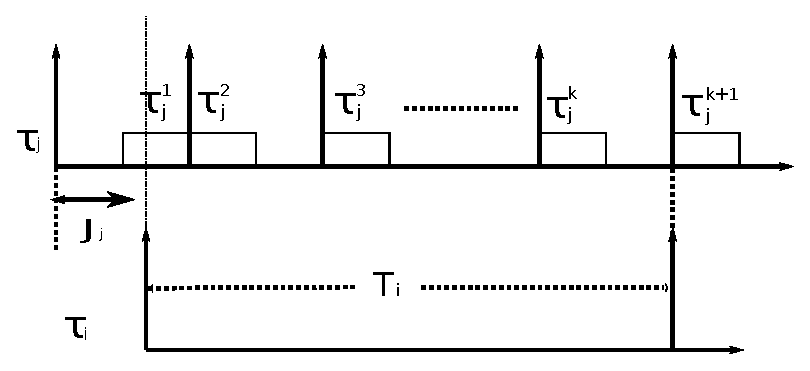
\includegraphics[bb=0bp 0bp 542bp 162bp,scale=0.5]{figures/figure9-a}
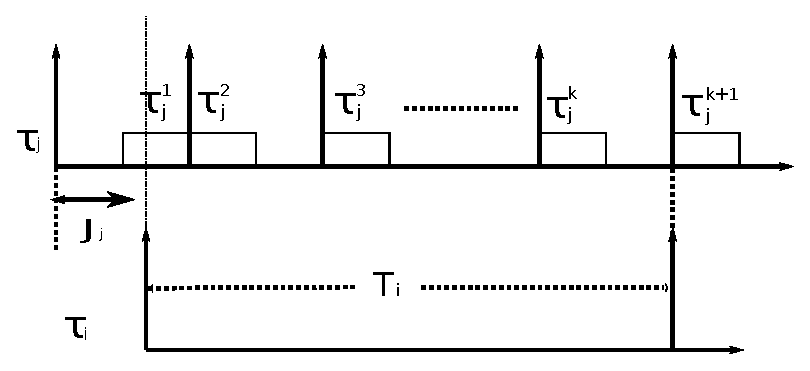
\includegraphics[scale=0.5]{figures/figure9-a}
\label{fig1}
}
%
\subfigure[during $L=T_i-f$, $f>b$]{
%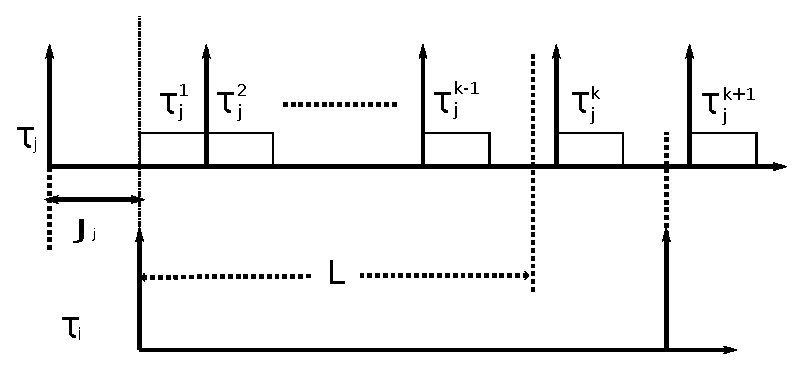
\includegraphics[bb=0bp 0bp 542bp 162bp,scale=0.5]{figures/figure9-b}
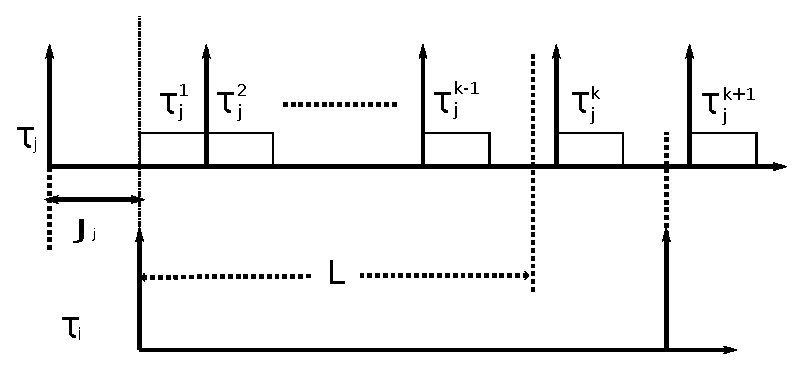
\includegraphics[scale=0.5]{figures/figure9-b}
\label{fig2}
}
%
\caption{Maximum interference of jobs of $\tau_j$ to $\tau_i^x$ running on different processors, under G-EDF. $T_i=aT_j+b$}
\label{fig:max_interference_gedf_j_i}
\end{figure}
%
\subsection{Retry Cost of Atomic Sections}
%
\begin{clm}\label{clm:basic_2_tx_rc}
Let $s_i^k$ and $s_j^l$ be two conflicting transactions. $s_i^k$ has a lower priority than $s_j^l$. Let the lower priority transaction always aborts and retries due to the higher priority transaction. $s_j^l$ interfere only once with $s_i^k$. $s_i^k$ aborts and retries due to $s_j^l$ for at most
%
\begin{equation}
len\left(s_i^k + s_j^l\right)\label{eq:basic_2_tx_rc}
\end{equation}
%
\end{clm}
%
\begin{proof}
%
$s_j^l$ must start at least when $s_i^k$ starts and not later than $s_i^k$ finishes. Otherwise, there will be no conflict between $s_i^k$ and $s_j^l$. $s_i^k$ must retry during execution of $s_j^l$ because of higher priority of $s_j^l$. The part of $s_i^k$ that started before beginning of $s_j^l$ will be repeated. Thus, the worst case interference between $s_i^k$ and $s_j^l$ occurs when $s_j^l$ starts just when $s_i^k$ reaches its end of execution. So, maximum retry cost of $s_i^k$ due to $s_j^l$ is calculated by~\ref{eq:basic_2_tx_rc}. Claim follows.
%
\end{proof}
%
\begin{clm}\label{clm:effect_one_tx_in_rc_multiple_txs}
%
Let conflict between transactions be resolved by priority (i.e., lower
priority transaction aborts and retries due to higher priority transactions).
Let $conf\left\{ s_{i}^{k}\right\} $ be the set of all transactions
that do not belong to any job of $\tau_{i}$ and are conflicting, directly or indirectly(transitively), with
$s_{i}^{k}$. Each transaction $s_{j}^{l}\in conf\left\{ s_{i}^{k}\right\} $
contributes to the retry cost of $s_{i}^{k}$ by at most 
\begin{equation}
len\left(s_{j}^{l}+max\_s_{ik}^{jl}(\Theta)\right)\label{eq:effect_one_tx_in_rc_multiple_txs}
\end{equation}
where $max\_s_{ik}^{jl}(\Theta)$ is the maximum length atomic section
(transaction) in $conf\{s_{i}^{k}\}$ that accesses $\Theta$ and its priority
is lower than $p(s_{j}^{l})$ and higher than or equal to $p(s_{i}^{k})$. $max\_s_{ik}^{jl} \not\in s_{j}$
and $\Theta\subseteq\Theta_{i}^{k^{ex}}\cap\Theta_{j}^{l}$.
%
\end{clm}
%
\begin{proof}
%
As conflict is resolved by transactional priority, then only transactions with higher priorities than $p(s_{i}^{k})$ will cause $s_{i}^{k}$ to abort and retry. Also, $s_j^l$ will abort only transactions with lower priority than $p(s_j^l)$. As transactions that belong to the same job execute sequentially, and jobs of the same task execute sequentially ,  so $s_i^k$ is not aborted by other transactions that belong to $\tau_i$. So, at any point of time after $s_{i}^{k}$ was first released, and before the last successful run of $s_i^k$ (i.e., the run at which $s_i^k$ commits), one of the following cases happens: 
\begin{enumerate}
\item $s_{j}^{l}$ has finished before $s_{i}^{k}$ starts. Or, $s_{j}^{l}$
starts after $s_{i}^{k}$ finishes. In this case, $s_{j}^{l}$ will
not cause $s_{i}^{k}$ to abort and retry. (\ref{eq:effect_one_tx_in_rc_multiple_txs})
still upper bounds effect of $s_{j}^{l}$ to the retry cost of $s_{i}^{k}$.
\item $s_{j}^{l}$ is the only transaction that is currently aborting $s_{i}^{k}$.
So, (\ref{eq:effect_one_tx_in_rc_multiple_txs}) follows directly
from Claim~\ref{clm:basic_2_tx_rc} as $len\left(s_{i}^{k}\right)\le len\left(max\_s_{ik}^{jl}(\Theta)\right)$. 
\item A set of transactions $S\subseteq conf\{s_{i}^{k}\}$ are currently
aborting $s_{i}^{k}$. $s_{j}^{l}\in S$ and $s_{j}^{l}$ itself is
not aborting and retrying due to any other transaction with higher
priority than $p(s_{j}^{l})$. So, $s_{j}^{l}$ executes only once.
$s_{j}^{l}$ aborts one of the transactions with lower priority than
$p(s_{j}^{l})$ for only once. Thus, (\ref{eq:effect_one_tx_in_rc_multiple_txs})
upper bounds effect of $s_{j}^{l}$ to the retry cost of $s_{i}^{k}$.
\item A set of transactions $S\subseteq conf\{s_{i}^{k}\}$ are currently
aborting $s_{i}^{k}$. $s_{j}^{l}\in S$ and $s_{j}^{l}$ itself is
aborting and retrying due to other transactions with higher priority
than $p(s_{j}^{l})$. Without losing generality, let $s_{h}^{u}$ be the transaction that is currently aborting $s_{j}^{l}$, and $s_{h}^{u}$
is not aborting and retrying due to any other higher priority transaction.
Then, $s_{j}^{l}$ and $s_{i}^{k}$ are both waiting for $s_{h}^{u}$
to finish. Thus, the time of retrial of $s_{j}^{l}$ due to $s_h^u$ is covered by effect of $s_{h}^{u}$ to the retry cost of $s_{i}^{k}$. When $s_{h}^{u}$ finishes and
$s_{j}^{l}$ is not aborted by any other higher priority transaction,
effect of $s_{j}^{l}$ to the retry cost of $s_{i}^{k}$ is the same
as in the third case. By expanding this case to more than three transactions,
then each transaction $s_{j}^{l}$ is either aborting one of the lower
priority transactions only once (i.e., the last successful run of $s_j^l$), or $s_{i}^{k}$ and
$s_{j}^{l}$ are aborted by a higher priority transaction $s_{h}^{u}$. When $s_j^l$ is retrying due to the higher priority transaction $s_h^u$, $s_j^l$ retrial time is not considered in retry cost of $s_i^k$ because it is already covered by the effect of the higher priority transaction $s_h^u$ to the retry cost of $s_i^k$.
\end{enumerate}
Claim follows.
\end{proof}
%
\begin{clm}\label{gedf-edf}
Under ECM, the total retry cost suffered by all transactions in any job $\tau_i^x \in \tau_i$ during interval $L \le T_i$ due to direct and indirect conflict with other transactions in jobs with higher priority than $\tau_i^x$ is upper bounded by:
%
\begin{equation}
RC_i\left(L\right) \le \sum_{\tau_{j}\in\gamma_i^{ex}}\left(g_{ij}^{gedf} \sum_{\forall s_j^l,\,\left(\Theta=\Theta_j^l \cap \Theta_i^{ex}\right) \neq \emptyset} len\left(s_{j}^{l} + s_{max}(\Theta)\right)\right)\label{eq3}\end{equation}
%
where $s_{max} \not\in s_j$ and $g_{ij}^{gedf}$ is calculated by (\ref{eq:gedf_max_job_no_interfer_j_i}).
\end{clm}
\begin{proof}\normalfont
%
ECM is used with G-EDF scheduler. Thus, $p(s_i^k)$ is a dynamic priority that depends on the absolute deadline of containing job $\tau_i^x$. So, $conf\left\{ s_i^k \right\}$ for any $s_i^k$ includes each transaction $s_j^l \not\in s_i$ where $\Theta_j^l \cap \Theta_i^{k^{ex}} \neq \emptyset$. The worst case retry cost of any $s_i^k$ occurs when $p(s_i^k)$ is the lowest priority among all other conflicting transactions during $T_i$. $g_{ij}^{gedf}$ is the maximum number of jobs of $\tau_j \in \gamma_i^{ex}$ that can interfere with one job of $\tau_j$. Following Claims~\ref{clm:gedf_max_job_no_interfer_j_i},~\ref{clm:basic_2_tx_rc} and~\ref{clm:effect_one_tx_in_rc_multiple_txs}, Claim follows.
\end{proof}
%
\begin{clm}\label{clm:rc_i_j_gedf_Ti_carry_in}
%
Under ECM, upper bound on total retry cost given by (\ref{eq3})
can be tightened by considering carried\_in job of each $\tau_{j}$
(i.e., $\tau_{j}^{in}$ where $r_{j}^{in}<r_{i}^{x}$ and $d_{j}^{in}<d_{i}^{x}$
as defined in~\cite{key-2}) conflicting with $\tau_{i}^{x}$ during
interval $L=T_{i}-f$, where $T_{i}=aT_{j}+b$, $a=\left\lfloor \frac{T_{i}}{T_{j}}\right\rfloor $
and $f\le b$. (\ref{eq3}) will be modified to 
\begin{equation}
%
RC_{i}(L)\le\begin{cases}
\sum_{\tau_{j}\in\gamma_{i}^{ex}}\left(\lambda_{1}\left(j\right)+\chi\left(i,j\right)\right) & ,f\le b\\
\sum_{\tau_{j}\in\gamma_{i}^{ex}}\left(\left(\left\lceil\frac{L}{T_{j}}\right\rceil+1\right)\sum_{\forall s_{j}^{l},\left(\Theta=\Theta_{i}^{ex}\cap\Theta_{j}^{l}\right)\neq\emptyset}len\left(s_{j}^{l}+s_{max}(\Theta)\right)\right) & ,Otherwise
\end{cases}
\label{eq:rc_i_j_gedf_Ti_carry_in}
%
\end{equation}
%
where
\begin{compactitem}
\item $s_{max}\not\in s_{j}$.
\item $\lambda_{1}\left(j\right)=\sum_{\forall s_{j}^{l}\in\left[d_{j}^{in}-\delta,d_{j}^{in}\right],\left(\Theta=\Theta_{i}^{ex}\cap\Theta_{j}^{l}\right)}len\left(s_{j}^{l^{*}}+s_{max}\left(\Theta\right)\right)$,
where $\delta=min\left(c_{j},b\right)$ and $s_{j}^{l^{*}}$ is the
part of $s_{j}^{l}$ that is contained in interval $\left[d_{j}^{in}-\delta,d_{j}^{in}\right]$.
\item $\chi\left(i,j\right)=\left\lfloor\frac{T_{i}}{T_{j}}\right\rfloor\sum_{\forall s_{j}^{l},\left(\Theta=\Theta_{i}^{ex}\cap\Theta_{j}^{l}\right)\neq\emptyset}len\left(s_{j}^{l}+s_{max}\left(\Theta\right)\right)$.
\end{compactitem}
\end{clm}
%
\begin{proof}
%
Following proof of Claim~\ref{clm:gedf_max_job_no_interfer_j_i},
maximum number of jobs of $\tau_{j}$ that can interfere with $\tau_{i}^{x}$
is $\left\lceil\frac{T_{i}}{T_{j}}\right\rceil$. By definition of
carried-in jobs~\cite{key-2} and G-EDF scheduler, there will be $\left\lfloor\frac{T_{i}}{T_{j}}\right\rfloor$
jobs of $\tau_{j}$ that exist by their whole periods $T_{j}$
in the interval $L$. Carried-in job of $\tau_{j}$ (i.e., $\tau_{j}^{in}$)
will exist by at most $\delta=min\left(c_{j},b\right)$ during
$L$. $\tau_{j}^{in}$ is delayed by its maximum jitter to give its
maximum contribution during $L$. Thus, $\tau_{j}^{in}$ starts execution
at $d_{j}^{in}-c_{j}$. Consequently, only transactions of $\tau_{j}^{in}$
that are contained in $\left[d_{j}^{in}-\delta,d_{j}^{in}\right]$
can exist in the interval $L$. Also, if transaction $s_{j}^{l}$
is partially contained in $\left[d_{j}^{in}-\delta,d_{j}^{in}\right]$,
only the part of $s_{j}^{l}$ contained in $\left[d_{j}^{in}-\delta,d_{j}^{in}\right]$
(i.e., $s_{j}^{l^{*}}$) can conflict with transactions in $\tau_{i}^{x}$.
$\lambda(j)$ stands for the retry cost of transactions in $\tau_{i}^{x}$
due to conflict with transactions of $\tau_{j}^{in}$. Whereas, $\chi(i,j)$
stands for the retry cost of transactions in $\tau_{i}^{x}$ due to
conflict with transactions of other jobs of $\tau_{j}$ (i.e., non
carried-in jobs). Combining the previous notions with Claim~\ref{gedf-edf},
Claim follows.
%
\end{proof}
%
Effect of transactions in carried\_in job is shown in Figure~\ref{fig10}.
%
\begin{figure}
\centering{}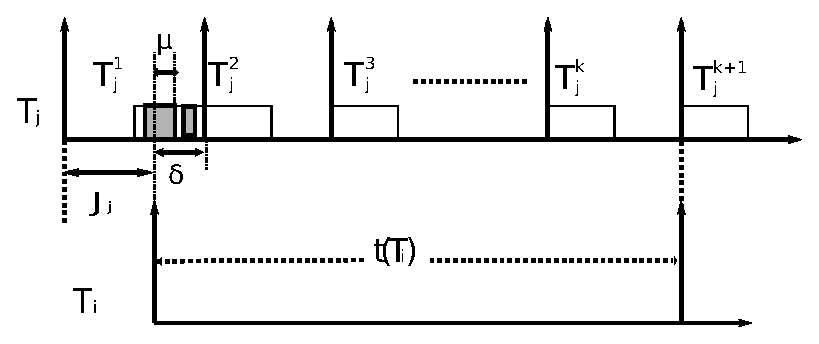
\includegraphics[scale=0.5]{figures/figure10}\caption{\label{fig10}Effect of carried\_in job of $\tau_j$ to retry cost of transactions in $\tau_i$}
\end{figure}
%
There are two sources of retry cost for any $\tau_i^x$ under ECM. First is due to conflict between $\tau_i^x$'s transactions and transactions of other jobs. This is denoted as $RC_i$. Second is due to the preemption of any transaction in $\tau_i^x$ due to the release of all higher priority jobs. This is denoted as $RC_{i_{re}}$. It is up to the implementation  of the contention manager to avoid $RC_{re}$. Here, as we are concerned with maximum total retry cost introduced by ECM, we assume that ECM does not avoid $RC_{re}$. Thus, we introduce $RC_{re}$ for ECM technique.
%
\begin{clm}\label{clm:ecm_release_conflict}
%
Under ECM, the total retry cost suffered by all transactions in any job $\tau_i^x \in \tau_i$ during an interval $L \le T_i$ due to release of jobs with higher priority than $\tau_i^x$ is upper bounded by 
\begin{equation}
RC_{i_{re}}(L) \le \sum_{\forall \tau_{j}\in\zeta_{i}}\begin{cases}
\left\lceil \frac{L}{T_{j}}\right\rceil s_{i_{max}} & ,L\le T_{i}-T_{j}\\\\
\left\lfloor \frac{T_{i}}{T_{j}}\right\rfloor s_{i_{max}} & ,L>T_{i}-T_{j}
\end{cases}\label{eq:ecm_release_conflict}
\end{equation}
%
where $\zeta_i=\{\tau_j:\left(\tau_j \ne \tau_i\right)\wedge \left(D_j < D_i \right)\}$.
\end{clm}
%
\begin{proof}
Two conditions must be satisfied for any $\tau_{j}^{l}$ to be able to preempt
$\tau_{i}^{x}$ under G-EDF: $r_{i}^{x}<r_{j}^{l}<d_{i}^{x}$,
and $d_{j}^{l}\le d_{i}^{x}$. Without the first condition, $\tau_{j}^{l}$
would have been already released before $\tau_{i}^{x}$. Thus, $\tau_j^l$ will
not preempt $\tau_i^x$. Without the second condition, $\tau_{j}^{l}$ will
be of lower priority than $\tau_{i}^{x}$ and will not preempt it.
If $D_{j} \ge D_{i}$, then there will be at most one instance $\tau_j^l$ with higher priority than $\tau_{i}^{x}$. $\tau_j^l$ must have been released at most at $r_i^x$, which violates the first condition. The other instance $\tau_j^{l+1}$ would have an absolute deadline greater than $d_i^x$. This violates the second condition. Hence, only tasks with shorter relative deadline than $D_{i}$ are considered. These jobs are grouped in $\zeta_i$.

The total number of released instances of $\tau_{j}$ during any interval $L\le T_{i}$ is $\left\lceil \frac{L}{T_{i}}\right\rceil +1$. The ``carried-in" jobs (i.e., each job released before $r_i^x$ and has an absolute deadline before $d_i^x$~\cite{key-2}) are discarded as they violate the first condition. The ``carried-out" jobs (i.e., each job released after $r_i^x$ and has an absolute deadline after $d_i^x$~\cite{key-2}) are also discarded because they violate the second condition. Thus, the number of considered higher priority instances of $\tau_j$ during the interval $L\le T_i-T_j$ is $\left\lceil\frac{L}{T_j}\right\rceil$. The number of considered higher priority instances of $\tau_j$ during interval $L> T_i-T_j$ is $\left\lfloor\frac{T_i}{T_j}\right\rfloor$.

The worst $RC_{i_{re}}$ for $\tau_i^x$ occurs when $\tau_i^x$ is always interfered at the end of execution of its longest atomic section, $s_{i_{max}}$. $\tau_i^x$ will have to retry for $len(s_{i_{max}})$. Claim follows.
\end{proof}
%
\begin{clm}\label{clm:ecm_total_rc}
Under ECM, the total retry cost suffered by all transactions in any job $\tau_i^x \in \tau_i$ during an interval $L\le T_i$ is upper bounded by:
\begin{equation}
RC_{i_{to}}(L)=RC_i(L)+RC_{i_{re}}(L)
\label{eq:ecm_total_rc}
\end{equation}
where $RC_i(L)$ is the maximum retry cost resulting from conflict between transactions in $\tau_i^x$ and transactions of other jobs. $RC_i(L)$ is calculated by (\ref{eq3}). $RC_{i_{re}}(L)$ is the maximum retry cost resulting from the release of higher priority jobs, which preempt transactions in $\tau_i^x$. $RC_{i_{re}}(L)$ is calculated by (\ref{eq:ecm_release_conflict}).
%
\end{clm}
\begin{proof}\normalfont
%
Under ECM, transactions in any job $\tau_i^x \in \tau_i$ retry due to: 1) conflicting transactions of jobs with higher priority than $\tau_i^x$. 2) release of higher priority jobs that preempt $\tau_i^x$. Thus, (\ref{eq:ecm_total_rc}) follows directly from Claims~\ref{clm:rc_i_j_gedf_Ti_carry_in} and~\ref{clm:ecm_release_conflict}. Claim follows.
%
\end{proof}
%
\subsection{Upper Bound on Response Time}
%
\begin{clm}\label{clm:ecm_response_time_upper_bound}
%
Under ECM, maximum response time of any job $\tau_i^x \in \tau_i$ is upper bounded by 
%
\begin{equation}
R_{i}^{up}=c_{i}+RC_{i_{to}}(R_i^{up})+\left\lfloor\frac{1}{m}\sum_{j\ne i}I_{ij}(R_{i}^{up})\right\rfloor
\label{eq10}
\end{equation}
%
where:
\begin{compactitem}
\item $R_{i}^{up}$'s initial value is $c_i + R_i^{up}(c_i)$.
\item $RC_{i_{to}}(R_i^{up})$ is calculated by (\ref{eq:ecm_total_rc}).
\item $c_j$ of any job $\tau_j^y \in \tau_j$- contributing to the retry cost of transactions in $\tau_i^x$- is modified to 
\begin{equation}
c_{ji}=c_{j}-\left(\sum_{s_j^l,\left(\Theta=\Theta_i^{ex} \cap \Theta_j^l\right)\neq \emptyset}len \left(s_j^l \right) \right)+RC_{{ji}_{to}}(R_i^{up})\label{eq9}\end{equation}
\item $RC_{{ji}_{to}}(R_i^{up})$ is the same as $RC_{j_{to}}(R_i^{up})$ excluding atomic sections in $\tau_j$ that access shared objects between $\tau_i$ and $\tau_j$. $\tau_i$ does not contribute to $RC_{j_{re}}(R_i^{up})$.
\item $I_{ij}(R_{i}^{up})$ is calculated by (\ref{eq13}) with $c_{j}$ replaced by 
$c_{ji}$ and changing~(\ref{eq12}) to 
\begin{equation}
I_{ij}(R_i^{up})=max\begin{cases}
\left(\left\lceil\frac{R_i^{up}-\left(c_{ji}+\sum_{s_j^l,\left(\Theta=\Theta_i^{ex} \cap \Theta_j^l\right)\neq \emptyset} len(s_j^l)\right)}{T_{j}}\right\rceil+1 \right)c_{ji}\\
\left\lceil\frac{R_i^{up}-c_{j}}{T_{j}}\right\rceil.c_{ji}+c_{j}-\sum_{s_j^l,\left(\Theta=\Theta_i^{ex} \cap \Theta_j^l\right)\neq \emptyset} {len(s_j^l)}\end{cases}\label{eq14}\end{equation}
\end{compactitem}
%
\end{clm}
%
\begin{proof}
%
To obtain an upper bound on the maximum response time (i.e., $R_i^{up}$) of any job $\tau_i^x$ of $\tau_{i}$, the term $RC_{i_{to}}(R_i^{up})$ must be added to the interference of other tasks during the non-atomic
execution of $\tau_{i}^x$. But this requires modification of the WCET of each
task as follows. 

$c_{j}$ of each interfering task $\tau_{j}$ should be inflated to accommodate the interference of each task $\tau_{k},$ $k\ne j,i$. Meanwhile, atomic regions that access shared objects between $\tau_{j}$ and $\tau_{i}$ should not be considered in the inflation cost, because they have already been calculated in $\tau_{i}$'s retry cost. As an upper bound on $R_i^{up}$ is calculated, then jobs of $\tau_j$ with higher priority than $\tau_i^x$ are only considered. Thus, $\tau_i^x$ has no contribution in $RC_{j_{re}}(R_i^{up})$. Thus, $\tau_{j}$'s inflated WCET becomes:
%
\begin{equation*}
c_{ji}=c_{j}-\left(\sum_{s_j^l,\left(\Theta=\Theta_i^{ex} \cap \Theta_j^l\right)\neq \emptyset}len \left(s_j^l \right) \right)+RC_{{ji}_{to}}(R_i^{up})
\end{equation*}
%
which is given by (~\ref{eq9}). $c_{ji}$ is the new WCET of $\tau_{j}$ relative to $\tau_{i}$. $\sum_{s_j^l,\left(\Theta=\Theta_i^{ex} \cap \Theta_j^l\right)\neq \emptyset} {len(s_j^l)}$ is the sum of lengths of all atomic sections in $\tau_{j}$ that access any object $\theta \in \Theta_i^{ex}$. $\sum_{s_j^l, \left(\Theta=\Theta_i^{ex} \cap \Theta_j^l\right)\neq \emptyset} \allowbreak {len(s_j^l)}$ is subtracted from $c_j$ because $\sum_{s_j^l,\left(\Theta=\Theta_i^{ex} \cap \Theta_j^l\right)\neq \emptyset} {len(s_j^l)}$ is already included in $RC_{i_{to}}(R_i^{up})$. $RC_{{ji}_{to}}(R_i^{up})$ is the $RC_{j_{to}}(R_i^{up})$ without including the shared objects between $\tau_{i}$ and $\tau_{j}$. The calculated WCET is relative to task $\tau_{i}$, as it changes from task to task. The upper bound on the response time of $\tau_{i}^x$, denoted $R_{i}^{up}$, can be calculated iteratively, by modifying (\ref{eq:gedf_response_time}), as follows:
\begin{equation*}
R_{i}^{up}=c_{i}+RC_{i_{to}}(R_i^{up})+\left\lfloor\frac{1}{m}\sum_{j\ne i}I_{ij}(R_{i}^{up})\right\rfloor
\end{equation*}
%
which is given by (\ref{eq10}). $R_{i}^{up}$'s initial value is $c_i + R_i^{up}(c_i)$.
%
$I_{ij}(R_{i}^{up})$ is calculated by (\ref{eq13}) with $c_{j}$ replaced by 
$c_{ji}$, and changing (\ref{eq12}) to
\begin{equation*}
I_{ij}(R_i^{up})=max\begin{cases}
\left(\left\lceil\frac{R_i^{up}-\left(c_{ji}+\sum_{s_j^l,\left(\Theta=\Theta_i^{ex} \cap \Theta_j^l\right)\neq \emptyset} len(s_j^l)\right)}{T_{j}}\right\rceil+1 \right)c_{ji}\\
\left\lceil\frac{R_i^{up}-c_{j}}{T_{j}}\right\rceil.c_{ji}+c_{j}-\sum_{s_j^l,\left(\Theta=\Theta_i^{ex} \cap \Theta_j^l\right)\neq \emptyset} {len(s_j^l)}\end{cases}\end{equation*}
%
as given by (\ref{eq14}). Eq(\ref{eq12}) is modified to (\ref{eq14}) because there are two cases for the first job of $\tau_j$ (i.e., $\tau_j^1$) contributing to the retry cost of $\tau_i^x$:

\textit{Case 1}. $\tau_j^1$ (shown in Figure~\ref{fig2}) contributes by $c_{ji}$. Thus, other instances of $\tau_j$ will begin after this modified WCET, but the sum of the shared objects' atomic section lengths is removed from $c_{ji}$, causing other instances to start earlier. Thus, the term $\sum_{s_j^l,\left(\Theta=\Theta_i^{ex} \cap \Theta_j^l\right)\neq \emptyset} {len(s_j^l)}$ is added to $c_{ji}$ to obtain the correct start time. 

\textit{Case 2}. $\tau_j^1$ contributes by its $c_j$, but the sum of the shared atomic section lengths  between $\tau_i$ and $\tau_j$ should be subtracted from the contribution of $\tau_j^1$, as they are already included in the retry cost. 

It should be noted that subtraction of $\sum_{s_j^l,\left(\Theta=\Theta_i^{ex} \cap \Theta_j^l\right)\neq \emptyset} {len(s_j^l)}$ is done in the first case to obtain the correct start time of other instances, while in the second case, this is done to get the correct contribution of $\tau_j^1$. The maximum is chosen from the two terms in (\ref{eq14}), because they differ in the contribution of their $\tau_j^1$s, and the number of instances after that. Claim follows.
%
\end{proof}
%
\section{RCM}
\label{sec:g-rma-rma-cm}
%
As G-RMA is a fixed priority scheduler,  a task $\tau_{i}$ will be interfered by those tasks with priorities higher than $\tau_{i}$ (i.e., $p_{j}>p_{i}$).  Upon a conflict, the RMA CM will commit the transaction that belongs to the higher priority task. Hereafter, we use \emph{RCM} to refer to a multicore system scheduled by G-RMA and resolves STM conflicts by the RMA CM. RCM is shown in Alogrithm~\ref{rcm_algorithm}.
\begin{algorithm}
\footnotesize{
\LinesNumbered
\KwData{$s_i^k\rightarrow$ interfered atomic section. $s_j^l\rightarrow$ interfering atomic section}
\KwResult{which atomic section aborts}
\eIf{$T_i < T_j$}
	{$s_j^l$ aborts\label{rcm:step_sicommits}\;}
	{$s_i^k$ aborts\label{rcm:step_siaborts}\;}
	}
\caption{RCM}
\label{rcm_algorithm}
\end{algorithm}

The same illustrative example in Section~\ref{ecm_illustrative_ex} is applied for RCM except that tasks' priorities are fixed.
%
\subsection{Maximum Task Interference}
%
Figure~\ref{fig11} illustrates the maximum interference caused by a task $\tau_{j}$
to a task $\tau_{i}$ under G-RMA. As $\tau_{j}$ is of higher priority than $\tau_{i}$,
$\tau_{j}^{k}$ will interfere with $\tau_{i}$ even if it is not totally
included in $T_{i}$. Unlike the G-EDF case shown in Figure~\ref{fig10}, 
where only the $\delta$ part of $\tau_{j}^{1}$ is considered, in G-RMA,
$\tau_{j}^{k}$ can contribute by the whole $c_{j}$, and all atomic
sections contained in $\tau_{j}^{k}$ must be considered. This is because, in G-EDF, the worst-case pattern releases $\tau_{i}^a$ before $d_{j}^{1}$
by $\delta$ time units, and $\tau_{i}^a$ cannot be interfered before it
is released. But in G-RMA, $\tau_{i}^a$ is already released, and can be
interfered by the whole $\tau_{j}^{k}$, even if this makes it infeasible.
%
\begin{figure}[htbp]
\centering
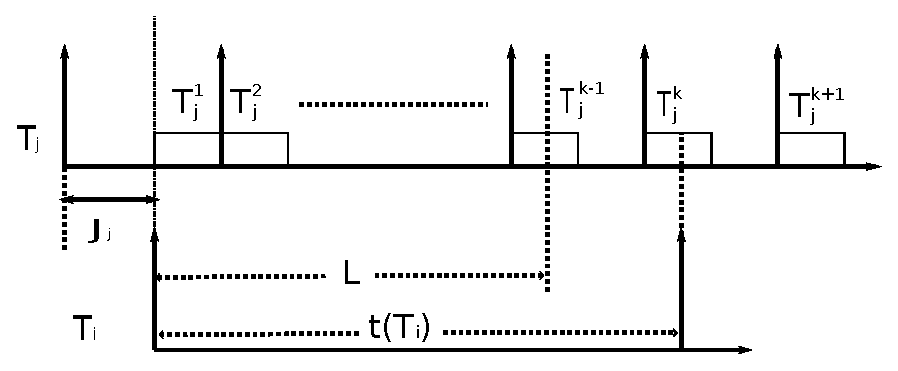
\includegraphics[scale=0.5]{figures/figure11}\caption{\label{fig11}Max interference of $\tau_{j}$ to $\tau_{i}$ in G-RMA}
\end{figure}

Thus, the maximum contribution of $\tau_{j}^b$ to $\tau_{i}^a$ for any duration
$L$ is upper bounded by Claim~\ref{clm:max_job_no_exist_j_interval_r}, where $L$ can extend to $T_{i}$. Note the contrast with ECM, where $L$ cannot be extended directly to $T_i$, as this will have a different pattern of worst case interference from other tasks.
%
\subsection{Retry Cost of Atomic Sections}
%
\begin{clm}\label{clm:rcm_retry_cost}
%
Under RCM, total retry cost suffered by all transactions in any job $\tau_i^x \in \tau_i$
during interval $L \le T_i$ due to direct and indirect conflict with other transactions in jobs with higher priorities than $\tau_i^x$ is upper bounded by:
% 
\begin{equation}
RC_i\left(L\right) \le \sum_{\tau_j \in \gamma_i^{ex},\,p_j > p_i}\left(\sum_{s_j^l,\left(\Theta=\Theta_i^{ex} \cap \Theta_j^l \right)\neq \emptyset}\left(\left(\left\lceil\frac{L}{T_{j}}\right\rceil+1\right)len\left(s_j^l+s_{max}\left(\Theta\right)\right)\right)\right)
\label{eq20}\end{equation} 
%
where $s_{max}\left(\Theta\right)$ belongs to a job with lower priority than $p_j$.
%
\end{clm}
%
\begin{proof}\normalfont
Under G-RMA, priorities of tasks are fixed. Thus, as $p_j > p_i$, then any job of $\tau_j$ will have a higher priority than $\tau_i^x$. So, Claim~\ref{clm:max_job_no_exist_j_interval_r} gives maximum number of jobs of $\tau_j$ that interfere with $\tau_i^x$ during interval $L$. By definition of RCM, only transactions with lower priority than $p_j$ can be aborted and retried due to transactions in $s_j$. Thus, $s_{max}\left(\Theta\right)$ cannot belong to transactions with priorities at least equal to $p_j$. Following proof of Claim~\ref{gedf-edf}, Claim follows.
%
\end{proof}
%
\begin{clm}\label{clm:rcm_release_conflict}
%
Under RCM, the total retry cost suffered by all transactions in any job $\tau_i^x \in \tau_i$ during an interval $L \le T_i$ due to release of jobs with higher priority than $\tau_i^x$ is upper bounded by 
%
\begin{equation}
RC_{i_{re}}(L)=\sum_{\forall \tau_j,\,p_j > p_i}\left(\left\lceil\frac{L}{T_j}\right\rceil s_{i_{max}}\right)\label{eq:rcm_release_conflict}
\end{equation}
%
\end{clm}
%
\begin{proof}
%
The proof is the same as that for Claim~\ref{clm:ecm_release_conflict}, except that G-RMA uses static priority. Thus, the carried-out jobs will be considered in the interference with $\tau_i^x$. The carried-in jobs are still not considered because they are released before $r_i^x$. Claim follows.
%
\end{proof}
%
\begin{clm}\label{clm:rcm_total_rc}
Under RCM, the total retry cost suffered by all transactions in any job $\tau_i^x \in \tau_i$ during an interval $L\le T_i$ is upper bounded by:
\begin{equation}
RC_{i_{to}}(L)=RC_i(L)+RC_{i_{re}}(L)
\label{eq:rcm_total_rc}
\end{equation}
where $RC_i(L)$ is the maximum retry cost resulting from conflict between transactions in $\tau_i^x$ and transactions of other jobs. $RC_i(L)$ is calculated by (\ref{eq20}). $RC_{i_{re}}(L)$ is the maximum retry cost resulting from the release of higher priority jobs, which preempt transactions in $\tau_i^x$. $RC_{i_{re}}(L)$ is calculated by (\ref{eq:rcm_release_conflict}).
%
\end{clm}
\begin{proof}\normalfont
%
Using Claims~\ref{clm:rcm_retry_cost} and~\ref{clm:rcm_release_conflict}, and following proof of Claim~\ref{clm:ecm_total_rc}, Claim follows.
%
\end{proof}
%
\subsection{Upper Bound on Response Time}
%
\begin{clm}\label{clm:rcm_response_time_upper_bound}
%
Under RCM, maximum response time of any job $\tau_i^x \in \tau_i$ is upper bounded by 
%
\begin{equation}
R_{i}^{up}=c_{i}+RC_{i_{to}}(R_i^{up})+\left\lfloor\frac{1}{m}\sum_{j\ne i, p_j > p_i}I_{ij}(R_{i}^{up})\right\rfloor
\label{eq:rcm_response_time_upper_bound}
\end{equation}
%
where:
\begin{compactitem}
\item $R_{i}^{up}$'s initial value is $c_i + R_i^{up}(c_i)$.
\item $RC_{i_{to}}(R_i^{up})$ is calculated by (\ref{eq:rcm_total_rc}).
\item $c_j$ of any job $\tau_j^y \in \tau_j$, where $p_j > p_i$ and $\Theta_j \cap \Theta_i^{ex} \neq \emptyset$, is calculated by (\ref{eq9}).
\item $I_{ij}(R_{i}^{up})$ is calculated by (\ref{eq12}) with $c_{j}$ replaced by 
$c_{ji}$.
\end{compactitem}
%
\end{clm}
%
\begin{proof}
%
Using Theorem 7 in~\cite{key-2}, Claim~\ref{clm:rcm_total_rc} and following proof of Claim~\ref{clm:ecm_response_time_upper_bound}, Claim follows.
%
\end{proof}
%
\section{STM versus Lock-Free}
\label{sec:comparison}
%
We now would like to understand when STM will be beneficial compared to lock-free synchronization. The retry-loop lock-free approach in~\cite{key-5} is the most relevant to our work. As lock-free instructions access only one object, then $\Theta_i^k$ for any $s_i^k$ will be restricted to one object only (i.e., $\Theta_i^k=\theta_i^k$). Thus, transitive retry cannot happen, $\Theta_i^{ex}=\Theta_i$ and $\gamma_i^{ex}=\gamma_i$.
%
\subsection{ECM versus Lock-Free}\label{sub:G-EDF-scheduler-with}
%
\begin{clm}\label{clm:ecm_lf_schedulability_cmp}
%
For ECM's schedulability to be better or equal to that of~\cite{key-5}'s retry-loop lock-free approach, the size of $s_{max}$ must not exceed one half of that of $r_{max}$, where $r_{max}$ is the maximum execution cost of a single iteration of any lock-free retry loop of any task. With equal periods for conflicting tasks and high access times to each object within the same transaction, the size of $s_{max}$ can be much larger than $r_{max}$.
%
\end{clm}
%
\begin{proof}\normalfont
%
Using Claim~\ref{clm:gedf_max_job_no_interfer_j_i}, (\ref{eq:rc_i_j_gedf_Ti_carry_in}) can be upper bounded, during $T_i$, as:
%
\begin{equation*}
RC_{i}^{max}\left(T_{i}\right) \le \sum_{\tau_{j}\in\gamma_{i}}\left(\left\lceil\frac{T_{i}}{T_{j}}\right\rceil\sum_{\forall s_{j}^{l}, \left(\Theta=\Theta_j^l \cap \Theta_i\right) \neq \emptyset}\left(2.s_{max}\right)\right)
\label{eq30}
\end{equation*}
%
where $s_{max}$ is the maximum length atomic section among all tasks. Similarly, (\ref{eq:ecm_release_conflict}) is upper bounded, during $T_i$, as:
%
\begin{equation*}
RC_{i_{re}}^{max} \le \sum_{\forall \tau_j \in \zeta_i} \left\lfloor \frac{T_i}{T_j}\right\rfloor s_{max}
\label{eq:ecm_release_conflict_stm_comp}
\end{equation*}
%
where $\zeta_i=\left\{ \tau_j : \left(\tau_j \neq \tau_i \right) \wedge \left( D_j < D_i \right)\right\}$. Thus, $RC_{i_{to}}$ given by (\ref{eq:ecm_total_rc}) can be upper bounded, during $T_i$, as:
\begin{equation}
RC_{i_{to}}^{max} \le \left(\sum_{\tau_{j}\in\gamma_{i}}\left(\left\lceil\frac{T_{i}}{T_{j}}\right\rceil\sum_{\forall s_{j}^{l}, \left(\Theta=\Theta_j^l \cap \Theta_i\right) \neq \emptyset}\left(2.s_{max}\right)\right)\right) +
\left( \sum_{\forall \tau_j \in \zeta_i} \left\lfloor \frac{T_i}{T_j}\right\rfloor s_{max} \right)
\label{eq:ecm_total_rc_stm_comp}
\end{equation}
%
Retry cost of $\tau_i$ during interval $T_i$ due to conflict with other jobs under retry-loop lock-free is given in~\cite{key-5} as:
%
\begin{equation}
LRC \le \sum_{\tau_{j}\in\gamma_{i}}\left(\left\lceil\frac{T_{i}}{T_{j}}\right\rceil+1\right).\beta_{ij}.r_{max}
\label{eq32}
\end{equation}
%
where $\beta_{ij}$ is the number of retry loops of $\tau_{j}$ that access shared objects between $\tau_{i}$ and $\tau_j$. (\ref{eq32}) needs to be extended to include effect of release of any higher priority job, $\tau_j^l$, preempting $\tau_i^k$ when $\tau_i^k$ is trying to access an object $\theta$. Release of jobs under ECM and lock-free is independent from accessed objects. Thus, ECM and lock-free have the same pattern of jobs' release. Thus,  retry cost of $\tau_i$ during $T_i$ due to release of higher priority jobs under retry-loop lock-free is obtained directly from Claim~\ref{clm:ecm_release_conflict} with replacing $s_{max}$ by $r_{max}$. Thus, total retry cost of any job of $\tau_i$ during interval $T_i$ due to conflict of other jobs and release of higher priority jobs is upper bounded by:
%
\begin{equation}
LRC_{to} \le \left(\left(\sum_{\tau_{j}\in\gamma_{i}}\left(\left\lceil\frac{T_{i}}{T_{j}}\right\rceil+1\right).\beta_{ij}\right) + \left(\sum_{\tau_j \in \zeta_i}\left\lfloor\frac{T_i}{T_j}\right\rfloor \right) \right) r_{max}
\label{eq:lf_total_rc}
\end{equation}
%
ECM achieves equal or better schedulability than lock-free if the total utilization under ECM is less than or equal to total utilization under lock-free system:
%
\begin{equation}
\sum_{\forall \tau_{i}}\frac{c_{i} + RC_{i_{to}}^{max}} {T_{i}} \le \sum_{\forall \tau_{i}}\frac{c_{i}+LRC_{to}}{T_{i}}
\label{eq:ecm_lf_util_cmp_1}
\end{equation}
%
Eq(\ref{eq:ecm_lf_util_cmp_1}) holds if for every task $\tau_i$:
%
\begin{equation}
RC_{i_{to}}^{max} \le LRC_{to}
\label{eq:ecm_lf_util_cmp_2}
\end{equation}
%
Thus,
\begin{eqnarray*}
 & \left(\left(\sum_{\forall\tau_{j}\in\gamma_{i}}\left(2\left\lceil \frac{T_{i}}{T_{j}}\right\rceil \sum_{\forall s_{j}^{l},\left(\Theta=\Theta_{j}^{l}\cap\Theta_{i}\right)\neq\emptyset}\right)\right)+\left(\sum_{\forall\tau_{j}\in\zeta_{i}}\left\lfloor \frac{T_{i}}{T_{j}}\right\rfloor \right)\right)s_{max}\\
\le & \left(\left(\sum_{\forall\tau_{j}\in\gamma_{i}}\left(\left\lceil \frac{T_{i}}{T_{j}}\right\rceil +1\right)\beta_{ij}\right)+\left(\sum_{\forall\tau_{j}\in\zeta_{i}}\left\lfloor \frac{T_{i}}{T_{j}}\right\rfloor \right)\right)r_{max}
\end{eqnarray*}
%
\begin{equation}
\therefore \frac{s_{max}}{r_{max}}\le\frac{\left(\sum_{\forall\tau_{j}\in\gamma_{i}}\left(\left\lceil \frac{T_{i}}{T_{j}}\right\rceil +1\right)\beta_{ij}\right)+\left(\sum_{\forall\tau_{j}\in\zeta_{i}}\left\lfloor \frac{T_{i}}{T_{j}}\right\rfloor \right)}{\left(\sum_{\forall\tau_{j}\in\gamma_{i}}\left(2\left\lceil \frac{T_{i}}{T_{j}}\right\rceil \sum_{\forall s_{j}^{l},\left(\Theta=\Theta_{j}^{l}\cap\Theta_{i}\right)\neq\emptyset}\right)\right)+\left(\sum_{\forall\tau_{j}\in\zeta_{i}}\left\lfloor \frac{T_{i}}{T_{j}}\right\rfloor \right)}
\label{eq:ecm_lf_util_cmp_3}
\end{equation}
%
Let $\sum_{\forall s_{j}^{l},\left(\Theta=\Theta_{j}^{l}\cap\Theta_{i}\right)\neq\emptyset}=\beta_{ij}^{*}$
and $\sum_{\forall\tau_{j}\in\zeta_{i}}\left\lfloor \frac{T_{i}}{T_{j}}\right\rfloor =c1$.
Then, (\ref{eq:ecm_lf_util_cmp_3}) becomes 
%
\begin{equation}
\frac{s_{max}}{r_{max}}\le\frac{\left(\sum_{\forall\tau_{j}\in\gamma_{i}}\left(\left\lceil \frac{T_{i}}{T_{j}}\right\rceil +1\right)\beta_{ij}\right)+c1}{\left(\sum_{\forall\tau_{j}\in\gamma_{i}}\left(2\left\lceil \frac{T_{i}}{T_{j}}\right\rceil \beta_{ij}^{*}\right)\right)+c1}
\label{eq:ecm_lf_util_cmp_4}
\end{equation}
%
We want to get the lower bound over $s_{max}/r_{max}$ that preserves equal or better schedulability for ECM than lock-free:

Each lock-free instruction accesses only one object once. Each transaction accesses only one object to enable comparison with lock-free. An object $\theta$ can be accessed multiple times within the same transaction. Thus, $\beta_{ij} \le \beta_{ij}^*$. 
\begin{equation*}
\because
\frac{\left(\sum_{\forall\tau_{j}\in\gamma_{i}}\left(\left\lceil \frac{T_{i}}{T_{j}}\right\rceil \right)\beta_{ij}^*\right) +c1}{\left(\sum_{\forall\tau_{j}\in\gamma_{i}}\left(2\left\lceil \frac{T_{i}}{T_{j}}\right\rceil \beta_{ij}^{*}\right)\right)+2c1} \le 
\frac{\left(\sum_{\forall\tau_{j}\in\gamma_{i}}\left(\left\lceil \frac{T_{i}}{T_{j}}\right\rceil +1\right)\beta_{ij}\right)+c1}{\left(\sum_{\forall\tau_{j}\in\gamma_{i}}\left(2\left\lceil \frac{T_{i}}{T_{j}}\right\rceil \beta_{ij}^{*}\right)\right)+c1}
\end{equation*}
%
Thus, (\ref{eq:ecm_lf_util_cmp_4}) holds if 
\begin{equation*}
\frac{s_{max}}{r_{max}} \le 
\frac{\left(\sum_{\forall\tau_{j}\in\gamma_{i}}\left\lceil \frac{T_{i}}{T_{j}}\right\rceil \beta_{ij}^*\right)+c1}{\left(\sum_{\forall\tau_{j}\in\gamma_{i}}\left(2\left\lceil \frac{T_{i}}{T_{j}}\right\rceil \beta_{ij}^{*}\right)\right)+2c1} = 
\frac{1}{2}
\end{equation*}
%
Thus, the lower bound over $s_{max}/r_{max}$ that preserves equal or better schedulability for ECM than lock-free is 0.5. Now, we want to get the upper bound over $s_{max}/r_{max}$ that preserves equal or better schedulability for ECM than lock-free:

Minimum value for $\left\lceil\frac{T_i}{T_j}\right\rceil$ is 1. So, $2\left\lceil\frac{T_i}{T_j}\right\rceil \ge \left\lceil\frac{T_i}{T_j}\right\rceil+1,\,\forall i,j$. Thus, to get upper bound on $s_{max}/r_{max}$, $\left\lceil\frac{T_i}{T_j}\right\rceil$ assumes its minimum value (i.e., 1). Otherwise, the denominator of (\ref{eq:ecm_lf_util_cmp_4}) gets larger than numerator, and $s_{max}/r_{max}$ moves away from its upper bound. $\left\lceil\frac{T_i}{T_j}\right\rceil \rightarrow 1$ for any $i,\,j$ if all conflicting tasks have equal periods. Thus, by substitution of $\left\lceil\frac{T_i}{T_j}\right\rceil=1$ into (\ref{eq:ecm_lf_util_cmp_4}), we get 
%
\begin{equation}
\frac{s_{max}}{r_{max}}\le\frac{\left(\sum_{\forall\tau_{j}\in\gamma_{i}}2\beta_{ij}\right)+c1}{\left(\sum_{\forall\tau_{j}\in\gamma_{i}}2 \beta_{ij}^{*}\right)+c1}
\label{eq:ecm_lf_util_cmp_5}
\end{equation}
%
As we are looking for the upper bound over $s_{max}/r_{max}$, then $\beta_{ij} >> \beta_{ij}^*$. Thus, $s_{max}$ can be much larger than $r_{max}$ while still maintaining equal or better schedulability for ECM than lock-free. From the previous notions, Claim follows.
%
\end{proof}
%
\subsection{RCM versus Lock-Free}\label{subsec:rcm_vs_lf}
%
\begin{clm}
%
For RCM's schedulability to be better or equal to that of~\cite{key-5}'s retry-loop lock-free approach, the size of $s_{max}$ must not exceed one half of that of $r_{max}$, where $r_{max}$ is the maximum execution cost of a single iteration of any lock-free retry loop of any task. With equal periods for conflicting tasks and high access times to each object within the same transaction, the size of $s_{max}$ can be much larger than $r_{max}$.
%
\end{clm}
%
\begin{proof}\normalfont
%
Following the same steps in proof of Claim~\ref{clm:ecm_lf_schedulability_cmp} with the following modifications:

Equation (\ref{eq20}) is upper bounded by:
%
\begin{equation}
\sum_{\tau_{j}\in\gamma_{i},\,p_{j}> p_{i}}\left(\sum_{s_j^l,\,\left(\Theta=\Theta_j^l \cap \Theta_i\right) \neq \emptyset}\left(\left(\left\lceil\frac{T_{i}}{T_{j}}\right\rceil+1\right)2s_{max}\right)\right)
\label{eq34}
\end{equation}
%
Equation (\ref{eq:rcm_release_conflict}) is upper bounded by:
%
\begin{equation}
RC_{i_{re}}(T_i)=\sum_{\forall \tau_j,\,p_j > p_i}\left(\left\lceil\frac{T_i}{T_j}\right\rceil s_{max}\right)
\label{eq:rcm_release_conflict_max}
\end{equation}
%
Thus, 
\begin{equation}
RC_{i_{to}}^{max} \le \sum_{\tau_{j}\in\gamma_{i},\,p_{j}> p_{i}}\left(\sum_{s_j^l,\,\left(\Theta=\Theta_j^l \cap \Theta_i\right) \neq \emptyset}\left(\left(\left\lceil\frac{T_{i}}{T_{j}}\right\rceil+1\right)2s_{max}\right)\right) + 
\sum_{\forall \tau_j,\,p_j > p_i}\left(\left\lceil\frac{T_i}{T_j}\right\rceil s_{max}\right)
\label{eq:rcm_rc_max_1}
\end{equation}
%
As lock-free is independent from the underlying scheduler, then $LRC$ is still calculated by (\ref{eq32}). Release of jobs under RCM and lock-free is independent from accessed objects. Thus, RCM and lock-free have the same pattern for object release. Thus, retry cost of transactions in $\tau_i$ during $T_i$ due to release of higher priority jobs under retry-loop lock-free is obtained directly from Claim~\ref{clm:rcm_release_conflict} with replacing $s_{max}$ by $r_{max}$. Thus,
%
\begin{equation}
LRC_{to} \le \left(\left(\sum_{\tau_{j}\in\gamma_{i}}\left(\left\lceil\frac{T_{i}}{T_{j}}\right\rceil+1\right).\beta_{ij}\right) + \left(\sum_{\tau_j,\,p_j > p_i}\left\lceil\frac{T_i}{T_j}\right\rceil \right) \right) r_{max}
\label{eq:lf_total_rc_grma}
\end{equation}
%
Similar to proof of Claim~\ref{clm:ecm_lf_schedulability_cmp}, RCM has equal or better schedulability than lock-free if for each $\tau_i$ 
%
\begin{equation}
\frac{s_{max}}{r_{max}}\le\frac{\left(\sum_{\forall\tau_{j}\in\gamma_{i}}\left(\left\lceil \frac{T_{i}}{T_{j}}\right\rceil +1\right)\beta_{ij}\right)+\left(\sum_{\forall\tau_{j},p_{j}>p_{i}}\left\lceil \frac{T_{i}}{T_{j}}\right\rceil \right)}{\left(\sum_{\forall\tau_{j}\in\gamma_{i},\,p_j>p_i}\left(2\left(\left\lceil \frac{T_{i}}{T_{j}}\right\rceil +1\right)\sum_{\forall s_{j}^{l},\left(\Theta=\Theta_{j}^{l}\cap\Theta_{i}\right)\neq\emptyset}\right)\right)+\left(\sum_{\forall\tau_{j},p_{j}>p_{i}}\left\lceil \frac{T_{i}}{T_{j}}\right\rceil \right)}
\label{eq:rcm_lf_comp_1}
\end{equation}
%
\begin{equation*}
\because \sum_{\forall\tau_{j}\in\gamma_{i},\,p_j>p_i}\left(2\left(\left\lceil \frac{T_{i}}{T_{j}}\right\rceil +1\right)\sum_{\forall s_{j}^{l},\left(\Theta=\Theta_{j}^{l}\cap\Theta_{i}\right)\neq\emptyset}\right) \le 
\sum_{\forall\tau_{j}\in\gamma_{i}}\left(2\left(\left\lceil \frac{T_{i}}{T_{j}}\right\rceil +1\right)\sum_{\forall s_{j}^{l},\left(\Theta=\Theta_{j}^{l}\cap\Theta_{i}\right)\neq\emptyset}\right)
\end{equation*} 
%
$\therefore$ Eq(\ref{eq:rcm_lf_comp_1}) holds if 
%
\begin{equation}
\frac{s_{max}}{r_{max}}\le\frac{\left(\sum_{\forall\tau_{j}\in\gamma_{i}}\left(\left\lceil \frac{T_{i}}{T_{j}}\right\rceil +1\right)\beta_{ij}\right)+\left(\sum_{\forall\tau_{j},p_{j}>p_{i}}\left\lceil \frac{T_{i}}{T_{j}}\right\rceil \right)}{\left(\sum_{\forall\tau_{j}\in\gamma_{i}}\left(2\left(\left\lceil \frac{T_{i}}{T_{j}}\right\rceil +1\right)\sum_{\forall s_{j}^{l},\left(\Theta=\Theta_{j}^{l}\cap\Theta_{i}\right)\neq\emptyset}\right)\right)+\left(\sum_{\forall\tau_{j},p_{j}>p_{i}}\left\lceil \frac{T_{i}}{T_{j}}\right\rceil \right)}
\label{eq:rcm_lf_comp_2}
\end{equation}
%
Let $\sum_{\forall s_{j}^{l},\left(\Theta=\Theta_{j}^{l}\cap\Theta_{i}\right)\neq\emptyset}=\beta_{ij}^{*}$
and $\sum_{\forall\tau_{j},p_{j}>p_{i}}\left\lceil \frac{T_{i}}{T_{j}}\right\rceil =c1$.
Then (\ref{eq:rcm_lf_comp_1}) becomes 
%
\begin{equation}
\frac{s_{max}}{r_{max}}\le\frac{\left(\sum_{\forall\tau_{j}\in\gamma_{i}}\left(\left\lceil \frac{T_{i}}{T_{j}}\right\rceil +1\right)\beta_{ij}\right)+c1}{\left(\sum_{\forall\tau_{j}\in\gamma_{i}}\left(2\left(\left\lceil \frac{T_{i}}{T_{j}}\right\rceil +1\right)\beta_{ij}^{*}\right)+c1\right)}
\label{eq:rcm_lf_comp_3}
\end{equation}
%
We want to get lower bound over $s_{max}/r_{max}$ that preserves equal or better schedulability for RCM than lock-free:

Similar to proof of Claim~\ref{clm:ecm_lf_schedulability_cmp}, $\beta_{ij}$ assumes its minimum value $\beta_{ij}^*$. 
%
\begin{equation}
\because\frac{\left(\sum_{\forall\tau_{j}\in\gamma_{i}}\left(\left\lceil \frac{T_{i}}{T_{j}}\right\rceil +1\right)\beta_{ij}\right)+c1}{\left(\sum_{\forall\tau_{j}\in\gamma_{i}}\left(2\left(\left\lceil \frac{T_{i}}{T_{j}}\right\rceil +1\right)\beta_{ij}^{*}\right)+2c1\right)}\le\frac{\left(\sum_{\forall\tau_{j}\in\gamma_{i}}\left(\left\lceil \frac{T_{i}}{T_{j}}\right\rceil +1\right)\beta_{ij}\right)+c1}{\left(\sum_{\forall\tau_{j}\in\gamma_{i}}\left(2\left(\left\lceil \frac{T_{i}}{T_{j}}\right\rceil +1\right)\beta_{ij}^{*}\right)+c1\right)}
\end{equation}
%
Then (\ref{eq:rcm_lf_comp_3}) holds if 
\begin{equation}
\frac{s_{max}}{r_{max}} \le 
\frac{\left(\sum_{\forall\tau_{j}\in\gamma_{i}}\left(\left\lceil \frac{T_{i}}{T_{j}}\right\rceil +1\right)\beta_{ij}\right)+c1}{\left(\sum_{\forall\tau_{j}\in\gamma_{i}}\left(2\left(\left\lceil \frac{T_{i}}{T_{j}}\right\rceil +1\right)\beta_{ij}^{*}\right)+2c1\right)} = \frac{1}{2}
\end{equation}
%
We want to get upper bound over $s_{max}/r_{max}$ that preserves equal or better schedulability for RCM than lock-free:

Similar to proof of Claim~\ref{clm:ecm_lf_schedulability_cmp}, $\left\lceil\frac{T_i}{T_j}\right\rceil$ assumes its minimum value (i.e., 1), $\beta_{ij} >> \beta_{ij}^*$. Thus, $s_{max}$ can be much larger than $r_{max}$. From the previous notions, Claim follows.
%
\end{proof}
%
\section{STM versus Locking protocols}\label{sec:stm_vs_locking}
%
Schedulabilty of different CMs is compared against real-time locking protocols (i.e., OMLP\cite{springerlink:10.1007/s10617-012-9090-1,key-3} and RNLP\cite{6257574}) using total utilization under G-EDF and G-RMA. In  \cite{springerlink:10.1007/s10617-012-9090-1,key-3,6257574,nurtlwib}, priority inversion bound (\textit{pi-blocking}) is considered part of each task's execution time. Thus, each task's WCET is inflated by \textit{pi-blocking} bounds. Similarly, under different CMs, each
task's WCET is inflated by its total retry cost (i.e., retry cost due to direct and indirect conflict with other tasks. Besides retry cost due to release of higher priority jobs). So, schedulability of a specific STM CM algorithm $A$ is compared against a real-time
locking protocol $B$ as follows:
%
\begin{eqnarray}
\sum_{\forall\tau_{i}}\frac{c_{i}+RC_{A}(T_{i})}{T_{i}} & \le & \sum_{\forall\tau_{i}}\frac{c_{i}+PI_{B}(T_{i})}{T_{i}}\label{eq:stm_vs_locking_protocol}
\end{eqnarray}
%
Eq(\ref{eq:stm_vs_locking_protocol}) holds if 
%
\begin{equation}
\forall\tau_{i},\, RC_{A}(T_{i}) \le PI_{B}(T_{i})\label{eq:job_stm_vs_locking_protocol}
\end{equation}
%
If $\tau_{i}$ has no critical sections, then $RC_{A}(T_{i})=PI_{B}(T_{i})=0$.
Thus, independent tasks have the same effect in (\ref{eq:stm_vs_locking_protocol})
and they will not be considered in (\ref{eq:job_stm_vs_locking_protocol}).
%
\subsection{Priority Inversion under Global OMLP}\label{subsec:pi_omlp}
%
Under Global OMLP\cite{springerlink:10.1007/s10617-012-9090-1,key-3},
$PI_{OMLP}(T_{i})$ for any job $\tau_{i}^{x}$ is upper bounded by 
%
\begin{equation}
PI_{OMLP}(T_{i})\le\sum_{k=1}^{n_{r}}N_{i,k}(2m-1)L_{max}\label{eq:pi_omlp}
\end{equation}
%
Where $n_{r}$ is total number of resources. $N_{i,k}$ is maximum
number of times resource $k$ is accessed by $\tau_{i}$. $L_{max}$
is the maximum length critical section in all tasks. Let $N_{i}=\sum_{k=1}^{n_{r}}N_{i,k}$,
which is the total number of critical sections in any job $\tau_{i}^{x}$.
Thus, (\ref{eq:pi_omlp}) becomes 
\begin{equation}
PI_{OMLP}(T_{i})\le N_{i}(2m-1)L_{max}\label{eq:pi_omlp-1}
\end{equation}
Let $N_{max}=max\left\{ N_{i}\right\}_{\forall i} $, $N_{min}=min\left\{ N_{i}\right\}_{\forall i} $,
$\Phi_{max}=max\left\lceil\frac{T_i}{T_j}\right\rceil_{\forall i,\,j}$. As independent tasks are not considered in (\ref{eq:job_stm_vs_locking_protocol}),
$\therefore\, N_{max},\, N_{min}\ge1$.

OMLP uses group locking to access multiple (i.e., nested) resources
in a critical section. Thus, to enable schedulability comparison between
OMLP and different CMs, it is assumed that each transaction (critical
section) accesses only one resource (i.e., $\Theta_i^k=\theta_i^k$). So, there will be no transitive retry in CMs. Thus, $\Theta_i^{ex}=\Theta_i$ and $\gamma_i^{ex}=\gamma_i$. Sections \ref{subsec:ecm_vs_rnlp} and~\ref{subsec:rcm_vs_rnlp} investigates comparison between different CMs and fine-grained locking protocols (i.e., RNLP) to access multiple resources within a critical section without group locking.
%
\subsection{ECM versus Global OMLP}\label{subsec:ecm_vs_omlp}
%
\begin{clm}\label{clm:ecm_vs_omlp}
%
Under globally scheduled systems, schedulability of ECM is equal or
better than schedulability of Global OMLP if 
\begin{eqnarray}
\frac{s_{max}}{L_{max}} & \le & \frac{N_{min}\left(2m-1\right)}{\left(2N_{max}+1\right)(n-1)\Phi_{max}}\label{eq:ecm_omlp_cmp_final}
\end{eqnarray}
%
\end{clm}
%
\begin{proof}
%
Substitute $RC_{A}(T_{i})$ and $PI_{B}(T_{i})$ in (\ref{eq:job_stm_vs_locking_protocol})
by (\ref{eq:ecm_total_rc_stm_comp}) and (\ref{eq:pi_omlp-1})
respectively. $\therefore$ (\ref{eq:job_stm_vs_locking_protocol})
holds if $\forall \tau_i$
%
\begin{eqnarray}
 & \left(\sum_{\tau_{j}\in\gamma_{i}}\left(\left\lceil\frac{T_{i}}{T_{j}}\right\rceil\sum_{\forall s_{j}^{l}, \left(\Theta=\Theta_j^l \cap \Theta_i\right) \neq \emptyset}\left(2.s_{max}\right)\right)\right) +
\left( \sum_{\forall \tau_j \in \zeta_i} \left\lfloor \frac{T_i}{T_j}\right\rfloor s_{max} \right) \nonumber \\
\le & N_{i}\left(2m-1\right)L_{max}\label{eq:ecm_omlp_cmp_1}
\end{eqnarray}
%	
Let $N_{i,j}=\sum_{\forall s_{j}^{l}, \left(\Theta=\Theta_j^l \cap \Theta_i\right) \neq \emptyset}$. As each transaction accesses only one object to enable comparison against OMLP, then $N_{i,j}$ is number of transactions in any job of $\tau_{j}$ conflicting with any transaction in any job of $\tau_{i}$. Thus, (\ref{eq:ecm_omlp_cmp_1}) becomes 
%
\begin{eqnarray}
 & \left(2\left(\sum_{\forall\tau_{j}\in\gamma_{i}}\left(\left\lceil \frac{T_{i}}{T_{j}}\right\rceil N_{i,j}\right)\right)+\left(\sum_{\forall\tau_{j}\in\zeta_{i}}\left\lfloor \frac{T_{i}}{T_{j}}\right\rfloor \right)\right)s_{max}\nonumber \\
\le & N_{i}\left(2m-1\right)L_{max}\label{eq:ecm_omlp_cmp_2}
\end{eqnarray}
%
\begin{eqnarray}
\therefore \frac{s_{max}}{L_{max}} & \le & \frac{N_{i}\left(2m-1\right)}{2\left(\sum_{\forall\tau_{j}\in\gamma_{i}}\left(\left\lceil \frac{T_{i}}{T_{j}}\right\rceil N_{i,j}\right)\right)+\left(\sum_{\forall\tau_{j}\in\zeta_{i}}\left\lfloor \frac{T_{i}}{T_{j}}\right\rfloor \right)}\label{eq:ecm_omlp_cmp_3}
\end{eqnarray}
%
Let $N_{max}=max\left\{ N_{i}\right\}_{\forall i} $, $N_{min}=min\left\{ N_{i}\right\}_{\forall i} $,
$\Phi_{max}=max\left\lceil\frac{T_i}{T_j}\right\rceil_{\forall i,\,j}$. According to definition of ECM, any $\tau_{j}\in\gamma_{i}$ also
belongs to $\zeta_{i}$. $\therefore\, n-1 \ge |\zeta_{i}|\ge|\gamma_{i}|$.
$\because\, N_{max}\ge N_{i,j}$, $N_{min}\le N_{i}$ and $\Phi_{max}\ge\left\lceil \frac{T_{i}}{T_{j}}\right\rceil \ge\left\lfloor \frac{T_{i}}{T_{j}}\right\rfloor $.
$\therefore$ Eq(\ref{eq:ecm_omlp_cmp_3}) holds if 
%
\begin{eqnarray}
\frac{s_{max}}{L_{max}} & \le & \frac{N_{min}\left(2m-1\right)}{2\left(\sum_{\forall\tau_{j}\in\zeta_{i}}\left(\Phi_{max}N_{max}\right)\right)+\left(\sum_{\forall\tau_{j}\in\zeta_{i}}\Phi_{max}\right)}\nonumber \\
 & \le & \frac{N_{min}\left(2m-1\right)}{\left(2N_{max}+1\right)(n-1)\Phi_{max}}\label{eq:ecm_omlp_cmp_4}
\end{eqnarray}
%
Claim follows.
%
\end{proof}
%
\subsection{RCM versus Global OMLP}\label{subsec:rcm_vs_omlp}
%
\begin{clm}\label{clm:rcm_vs_omlp}
%
Under globally scheduled systems, schedulability of RCM is equal or
better than schedulability of Global OMLP if 
\begin{eqnarray}
\frac{s_{max}}{L_{max}} & \le & \frac{N_{min}\left(2m-1\right)}{\left(2\left(\Phi_{max}+1\right)N_{max}+\Phi_{max}\right)(n-1)}\label{eq:rcm_omlp_cmp_final}
\end{eqnarray}
%
\end{clm}
%
\begin{proof}
%
Substitute $RC_{A}(T_{i})$ in (\ref{eq:job_stm_vs_locking_protocol})
by (\ref{eq:rcm_rc_max_1}) and follow the same steps in proof of Claim~\ref{clm:ecm_vs_omlp}. Claim follows.
%
\end{proof}
%
\subsection{Priority Inversion under RNLP}\label{subsec:pi_rnlp}
%
Under RNLP\cite{6257574} for global scheduling and \textit{I-KGLP} token lock (introduced as $R^2DGLP$ in \cite{6300160}), $PI_{RNLP}(T_{i})$ for any job $\tau_{i}^{x}$ is upper bounded by $\left(2m-1\right)L_{max}$ for each outermost request, where $L_{max}$ is the maximum length
of any outermost request. Thus, if $N_{i}$ is total number of outermost critical sections in any job of $\tau_{i}$, then 
%
\begin{equation}
PI_{RNLP}(T_{i})=N_{i}(2m-1)L_{max}
\label{eq:rnlp_pi}
\end{equation}
%
Let $N_{max}=max\left\{ N_{i}\right\}_{\forall i} $, $N_{min}=min\left\{ N_{i}\right\}_{\forall i} $,
$\Phi_{max}=max\left\lceil\frac{T_i}{T_j}\right\rceil$. As independent tasks are not considered in (\ref{eq:job_stm_vs_locking_protocol}),
$\therefore\, N_{max},\, N_{min}\ge1$.

In contrast to OMLP, RNLP supports nesting of objects. Thus, each object can be accessed individually without being grouped with other objects in the same critical section. So, in comparison between different CMs and RNLP, each transaction can access multiple objects.
%
\subsection{ECM versus RNLP}\label{subsec:ecm_vs_rnlp}
%
\begin{clm}\label{clm:ecm_vs_rnlp}
%
Under globally scheduled systems, schedulability of ECM is equal or
better than schedulability of RNLP if 
%
\begin{eqnarray}
\frac{s_{max}}{L_{max}} & \le & \frac{N_{min}\left(2m-1\right)}{\left(2N_{max}+1\right)(n-1)\Phi_{max}}\label{eq:ecm_rnlp_cmp_final}
\end{eqnarray}
%
\end{clm}
%
\begin{proof}
%
Substitute $RC_{A}(T_{i})$ and $PI_{B}(T_{i})$ in (\ref{eq:job_stm_vs_locking_protocol})
by (\ref{eq:ecm_total_rc_stm_comp}) and (\ref{eq:rnlp_pi}) respectively. $\therefore$ (\ref{eq:job_stm_vs_locking_protocol}) becomes 
%
\begin{eqnarray}
 & \left(\sum_{\tau_{j}\in\gamma_{i}^{ex}}\left(\left\lceil\frac{T_{i}}{T_{j}}\right\rceil\sum_{\forall s_{j}^{l}, \left(\Theta=\Theta_j^l \cap \Theta_i^{ex}\right) \neq \emptyset}\left(2s_{max}\right)\right)\right) +
\left( \sum_{\forall \tau_j \in \zeta_i} \left\lfloor \frac{T_i}{T_j}\right\rfloor s_{max} \right) \nonumber \\
\le & N_{i}\left(2m-1\right)L_{max}\label{eq:ecm_rnlp_cmp_1}
\end{eqnarray}
%
where $\gamma_i$ is replaced by $\gamma_i^{ex}$ and $\Theta_i$ is replaced by $\Theta_i^{ex}$ because each transaction can access multiple objects. So, transitive retry exists. Following the same steps of proof of Claim~\ref{clm:ecm_vs_omlp}, Claim follows.
%
\end{proof}
%
\subsection{RCM vs. RNLP}\label{subsec:rcm_vs_rnlp}
%
\begin{clm}\label{clm:rcm_vs_rnlp}
%
Under globally scheduled systems, schedulability of RCM is equal or
better than schedulability of RNLP if 
\begin{eqnarray}
\frac{s_{max}}{L_{max}} & \le & \frac{N_{min}\left(2m-1\right)}{\left(2\left(\Phi_{max}+1\right)N_{max}+\Phi_{max}\right)(n-1)}
\label{eq:rcm_rnlp_cmp_final}
\end{eqnarray}
%
\end{clm}
%
\begin{proof}
%
Substitute $RC_{A}(T_{i})$ in (\ref{eq:job_stm_vs_locking_protocol})
by (\ref{eq:rcm_rc_max_1}). $\gamma_i$ is replaced with $\gamma_i^{ex}$ and $\Theta_i$ is replaced with $\Theta_i^{ex}$ because transitive retry exists. Following the same steps of proof of Claim~\ref{clm:ecm_vs_omlp}, Claim follows.
%
\end{proof}
%
\section{Conclusions}
\label{sec:ecm-rcm-conclusions}
%
ECM and RCM use jobs' priorities to resolve conflicts between transactions. The transaction with lower priority aborts and retries due to the transaction with higher priority. As each transaction can access multiple objects, a transaction may abort indirectly due to another transaction with no shared objects between them. The indirect retrial is denoted as transitive retry. Under both ECM and RCM, a task incurs at most $2s_{max}$ retry cost for each of its atomic sections due to a conflict with another task's atomic section. Transactions can also retry due to release of higher priority jobs that preempt a transaction in a lower priority job. 

The $s_{max}/r_{max}$ ratio determines whether STM is better or as good as lock-free. ECM and RCM have equal or better schedulability than retry-loop lock-free if $s_{max}$ does not exceed one half of $r_{max}$. $s_{max}$ can exceed $r_{max}$ with equal periods between conflicting tasks, and large access times to the same object within the same transaction.

Schedulability of ECM and RCM was compared against real-time locking protocols (i.e., Global OMLP and RNLP). ECM have equal or better schedulability than OMLP and RNLP if 
%
$
\frac{s_{max}}{L_{max}} \le \frac{N_{min}\left(2m-1\right)}{\left(2N_{max}+1\right)(n-1)\Phi_{max}}
$ .
%
RCM have equal or better schedulability than OMLP and RNLP if 
$
\frac{s_{max}}{L_{max}} \le \frac{N_{min}\left(2m-1\right)}{\left(2\left(\Phi_{max}+1\right)N_{max}+\Phi_{max}\right)(n-1)}
$